
%% Beginning of file 'sample63.tex'
%%
%% Modified 2019 June
%%
%% This is a sample manuscript marked up using the
%% AASTeX v6.3 LaTeX 2e macros.
%%
%% AASTeX is now based on Alexey Vikhlinin's emulateapj.cls 
%% (Copyright 2000-2015).  See the classfile for details.

%% AASTeX requires revtex4-1.cls (http://publish.aps.org/revtex4/) and
%% other external packages (latexsym, graphicx, amssymb, longtable, and epsf).
%% All of these external packages should already be present in the modern TeX 
%% distributions.  If not they can also be obtained at www.ctan.org.

%% The first piece of markup in an AASTeX v6.x document is the \documentclass
%% command. LaTeX will ignore any data that comes before this command. The 
%% documentclass can take an optional argument to modify the output style.
%% The command below calls the preprint style which will produce a tightly 
%% typeset, one-column, single-spaced document.  It is the default and thus
%% does not need to be explicitly stated.
%%
%%
%% using aastex version 6.3
\documentclass{aastex63}

%% The default is a single spaced, 10 point font, single spaced article.
%% There are 5 other style options available via an optional argument. They
%% can be invoked like this:
%%
%% \documentclass[arguments]{aastex63}
%% 
%% where the layout options are:
%%
%%  twocolumn   : two text columns, 10 point font, single spaced article.
%%                This is the most compact and represent the final published
%%                derived PDF copy of the accepted manuscript from the publisher
%%  manuscript  : one text column, 12 point font, double spaced article.
%%  preprint    : one text column, 12 point font, single spaced article.  
%%  preprint2   : two text columns, 12 point font, single spaced article.
%%  modern      : a stylish, single text column, 12 point font, article with
%% 		  wider left and right margins. This uses the Daniel
%% 		  Foreman-Mackey and David Hogg design.
%%  RNAAS       : Preferred style for Research Notes which are by design 
%%                lacking an abstract and brief. DO NOT use \begin{abstract}
%%                and \end{abstract} with this style.
%%
%% Note that you can submit to the AAS Journals in any of these 6 styles.
%%
%% There are other optional arguments one can invoke to allow other stylistic
%% actions. The available options are:
%%
%%   astrosymb    : Loads Astrosymb font and define \astrocommands. 
%%   tighten      : Makes baselineskip slightly smaller, only works with 
%%                  the twocolumn substyle.
%%   times        : uses times font instead of the default
%%   linenumbers  : turn on lineno package.
%%   trackchanges : required to see the revision mark up and print its output
%%   longauthor   : Do not use the more compressed footnote style (default) for 
%%                  the author/collaboration/affiliations. Instead print all
%%                  affiliation information after each name. Creates a much 
%%                  longer author list but may be desirable for short 
%%                  author papers.
%% twocolappendix : make 2 column appendix.
%%   anonymous    : Do not show the authors, affiliations and acknowledgments 
%%                  for dual anonymous review.
%%
%% these can be used in any combination, e.g.
%%
%% \documentclass[twocolumn,linenumbers,trackchanges]{aastex63}
%%
%% AASTeX v6.* now includes \hyperref support. While we have built in specific
%% defaults into the classfile you can manually override them with the
%% \hypersetup command. For example,
%%
%% \hypersetup{linkcolor=red,citecolor=green,filecolor=cyan,urlcolor=magenta}
%%
%% will change the color of the internal links to red, the links to the
%% bibliography to green, the file links to cyan, and the external links to
%% magenta. Additional information on \hyperref options can be found here:
%% https://www.tug.org/applications/hyperref/manual.html#x1-40003
%%
%% Note that in v6.3 "bookmarks" has been changed to "true" in hyperref
%% to improve the accessibility of the compiled pdf file.
%%
%% If you want to create your own macros, you can do so
%% using \newcommand. Your macros should appear before
%% the \begin{document} command.
%%
\newcommand{\vdag}{(v)^\dagger}
\newcommand\aastex{AAS\TeX}
\newcommand\latex{La\TeX}

%% Reintroduced the \received and \accepted commands from AASTeX v5.2
%\received{June 1, 2019}
%\revised{January 10, 2019}
%% Command to document which AAS Journal the manuscript was submitted to.
%% Adds "Submitted to " the argument.
\submitjournal{AJ}

%% For manuscript that include authors in collaborations, AASTeX v6.3
%% builds on the \collaboration command to allow greater freedom to 
%% keep the traditional author+affiliation information but only show
%% subsets. The \collaboration command now must appear AFTER the group
%% of authors in the collaboration and it takes TWO arguments. The last
%% is still the collaboration identifier. The text given in this
%% argument is what will be shown in the manuscript. The first argument
%% is the number of author above the \collaboration command to show with
%% the collaboration text. If there are authors that are not part of any
%% collaboration the \nocollaboration command is used. This command takes
%% one argument which is also the number of authors above to show. A
%% dashed line is shown to indicate no collaboration. This example manuscript
%% shows how these commands work to display specific set of authors 
%% on the front page.
%%
%% For manuscript without any need to use \collaboration the 
%% \AuthorCollaborationLimit command from v6.2 can still be used to 
%% show a subset of authors.
%
%\AuthorCollaborationLimit=2
%
%% will only show Schwarz & Muench on the front page of the manuscript
%% (assuming the \collaboration and \nocollaboration commands are
%% commented out).
%%
%% Note that all of the author will be shown in the published article.
%% This feature is meant to be used prior to acceptance to make the
%% front end of a long author article more manageable. Please do not use
%% this functionality for manuscripts with less than 20 authors. Conversely,
%% please do use this when the number of authors exceeds 40.
%%
%% Use \allauthors at the manuscript end to show the full author list.
%% This command should only be used with \AuthorCollaborationLimit is used.

%% The following command can be used to set the latex table counters.  It
%% is needed in this document because it uses a mix of latex tabular and
%% AASTeX deluxetables.  In general it should not be needed.
%\setcounter{table}{1}

%%%%%%%%%%%%%%%%%%%%%%%%%%%%%%%%%%%%%%%%%%%%%%%%%%%%%%%%%%%%%%%%%%%%%%%%%%%%%%%%
%%
%% The following section outlines numerous optional output that
%% can be displayed in the front matter or as running meta-data.
%%
%% If you wish, you may supply running head information, although
%% this information may be modified by the editorial offices.
\shorttitle{Research Assignement}
\shortauthors{Masini}
\date{May 6, 2020}
%%
%% You can add a light gray and diagonal water-mark to the first page 
%% with this command:
%% \watermark{text}
%% where "text", e.g. DRAFT, is the text to appear.  If the text is 
%% long you can control the water-mark size with:
%% \setwatermarkfontsize{dimension}
%% where dimension is any recognized LaTeX dimension, e.g. pt, in, etc.
%%
%%%%%%%%%%%%%%%%%%%%%%%%%%%%%%%%%%%%%%%%%%%%%%%%%%%%%%%%%%%%%%%%%%%%%%%%%%%%%%%%
\graphicspath{{./}{figures/}}
%% This is the end of the preamble.  Indicate the beginning of the
%% manuscript itself with \begin{document}.

\begin{document}

\title{Dark Matter Halo : the behavior under tidial forces in M33 }

%% LaTeX will automatically break titles if they run longer than
%% one line. However, you may use \\ to force a line break if
%% you desire. In v6.3 you can include a footnote in the title.

%% A significant change from earlier AASTEX versions is in the structure for 
%% calling author and affiliations. The change was necessary to implement 
%% auto-indexing of affiliations which prior was a manual process that could 
%% easily be tedious in large author manuscripts.
%%
%% The \author command is the same as before except it now takes an optional
%% argument which is the 16 digit ORCID. The syntax is:
%% \author[xxxx-xxxx-xxxx-xxxx]{Author Name}
%%
%% This will hyperlink the author name to the author's ORCID page. Note that
%% during compilation, LaTeX will do some limited checking of the format of
%% the ID to make sure it is valid. If the "orcid-ID.png" image file is 
%% present or in the LaTeX pathway, the OrcID icon will appear next to
%% the authors name.
%%
%% Use \affiliation for affiliation information. The old \affil is now aliased
%% to \affiliation. AASTeX v6.3 will automatically index these in the header.
%% When a duplicate is found its index will be the same as its previous entry.
%%
%% Note that \altaffilmark and \altaffiltext have been removed and thus 
%% can not be used to document secondary affiliations. If they are used latex
%% will issue a specific error message and quit. Please use multiple 
%% \affiliation calls for to document more than one affiliation.
%%
%% The new \altaffiliation can be used to indicate some secondary information
%% such as fellowships. This command produces a non-numeric footnote that is
%% set away from the numeric \affiliation footnotes.  NOTE that if an
%% \altaffiliation command is used it must come BEFORE the \affiliation call,
%% right after the \author command, in order to place the footnotes in
%% the proper location.
%%
%% Use \email to set provide email addresses. Each \email will appear on its
%% own line so you can put multiple email address in one \email call. A new
%% \correspondingauthor command is available in V6.3 to identify the
%% corresponding author of the manuscript. It is the author's responsibility
%% to make sure this name is also in the author list.
%%
%% While authors can be grouped inside the same \author and \affiliation
%% commands it is better to have a single author for each. This allows for
%% one to exploit all the new benefits and should make book-keeping easier.
%%
%% If done correctly the peer review system will be able to
%% automatically put the author and affiliation information from the manuscript
%% and save the corresponding author the trouble of entering it by hand.


\author{Adrien Masini}
\affiliation{University of Arizona\\
Tucson, Az 85719, USA}

\collaboration{1}{(LaTeX collaboration)}

%\nocollaboration{2}

%% Note that the \and command from previous versions of AASTeX is now
%% depreciated in this version as it is no longer necessary. AASTeX 
%% automatically takes care of all commas and "and"s between authors names.

%% AASTeX 6.3 has the new \collaboration and \nocollaboration commands to
%% provide the collaboration status of a group of authors. These commands 
%% can be used either before or after the list of corresponding authors. The
%% argument for \collaboration is the collaboration identifier. Authors are
%% encouraged to surround collaboration identifiers with ()s. The 
%% \nocollaboration command takes no argument and exists to indicate that
%% the nearby authors are not part of surrounding collaborations.

%% Mark off the abstract in the ``abstract'' environment. 
\begin{abstract}

The topic we are studying here is the behavior of Dark Matter halo due to mass loss.
\vspace{0.5mm}
Understanding this behavior can help us understand how galaxies evolve and a better comprehension of dark matter itself.
\vspace{0.5mm}
How does dark matter behave under the influence of tidal forces ?
\vspace{0.5mm}
We do not know much about dark matter and there is still a lot to discover about it. Especially what it is and the properties it has.
\vspace{0.5mm}
In this study, we found that the density profile of M33's halo looks like a Hernquist profile until the point when the merger MW-M31 exert the greatest gravitational force on the halo. Then it start loosing mass mostly in the center. As we get further from the center, the trend looks similar as Hernquist profile.
\vspace{0.5mm}
That first means that dark matter halos react to strong gravitational field in the same way as Baryonnic matter does. Also, we will be exploring cored theory in more details to explain what happens.



\end{abstract}

%% Keywords should appear after the \end{abstract} command. 
%% See the online documentation for the full list of available subject
%% keywords and the rules for their use.
\keywords{Galaxy, Galaxy evolution, Local Group, Hernquist Profile, Dark matter halo, galaxy merger}

%% From the front matter, we move on to the body of the paper.
%% Sections are demarcated by \section and \subsection, respectively.
%% Observe the use of the LaTeX \label
%% command after the \subsection to give a symbolic KEY to the
%% subsection for cross-referencing in a \ref command.
%% You can use LaTeX's \ref and \label commands to keep track of
%% cross-references to sections, equations, tables, and figures.
%% That way, if you change the order of any elements, LaTeX will
%% automatically renumber them.
%%
%% We recommend that authors also use the natbib \citep
%% and \citet commands to identify citations.  The citations are
%% tied to the reference list via symbolic KEYs. The KEY corresponds
%% to the KEY in the \bibitem in the reference list below. 

\section{Introduction} \label{sec:intro}

The behavior of the dark matter halo in M33 due to the tidal forces caused by MW and M31 is yet to be understood. M33 is a spiral galaxy, third most massive member of the local group with the Milky Way (MW) and Andromeda (M31). It is believed that M33 is a satellite of M31 because it is gravitationally bound to the Andromeda galaxy. In detail, we will quantify and plot the evolution of M33's dark matter halo while it orbits the MW-M31 system. Specifically, I will study the change in M33’s dark matter profile owing to mass loss from tides and quantify the mass loss rate as a function of time.
\vspace{1.5mm}

According to the definition from \cite{Will12} a packet of stars hold together by more than baryon matter and gravitation define a galaxy. Baryon matter means gas and stars. So a galaxy also bound stars with dark matter. Galaxy evolution is defined by the modification of the morphology and/or the internal dynamics due to collision, star age or the super massive black hole in the center  \citep{Will12}. The local group describes galaxies bound together by gravity and is composed of two major spiral galaxies Andromeda (M31) and the Milky Way (MW). A Hernquist profile is an analytic model shown by Lars Hernquist in 1990\citep{Hern90}. Dark matter halo represent all the dark matter that is tidaly bound to a galaxy. A galaxy merger is a new system of galaxies that has collided and are now bound to form a bigger galaxy.
\vspace{1.5mm}

Dark matter play an important role in galaxy formation and evolution. The depth of the potential well is increased by Dark Matter, which allow the galaxy to form stars by accretion of gas. Dark matter halo merge to form bigger structures, but as they merge, the smaller halo is not necessarily absorbed immediately and can become a sub-halo of the all structure \citep{Delos19}. This phenomenon is due to "Violent relaxation", defined from \cite{Bell67} as a loss in the equilibrium of the system. The potential evolve due to a redistribution of the gravitational forces that makes the kinetic energy of the stars chaotic.
By studying how the density profile of a satellite sub-halo of smaller size evolves due to tidal forces, we will be able to understand how dark matter mass loss impacts how galaxies are able to retain their baryonic matter. Since most of the mass comes from the dark matter halo, if it is tydaly removed, it is easier for the baryonic matter to escape.
We would be able to predict how a subhalo merge with a larger Dark Matter halo by understanding the evolution of the mass profile of dark matter due to tidal forces.
Figure 1 below shows the density profile of a Dark Matter Halo as a function of radius at different times. This study did not take into account the dynamical friction between  the small sub-halo and the larger halo that merged together. We will also ignore friction in our analysis. In this figure we can see how the density profile of a Dark Matter halo is distributed without any tidal forces acting on it. This model will be helpful to compare the result we get under tidal forces and owing to mass loss.
We know almost nothing about the behavior of Dark Matter except that even though we cannot see it, it interacts with normal matter via gravity. That property will allow us to predict the behavior of Dark Matter structure as the galaxies and halos merge during a collision using a simulation. Also, \cite{Wechsler18} describes well how galaxies and dark matter halos are connected. 

\vspace{0.5mm}

\begin{figure}[h]
    \centering
    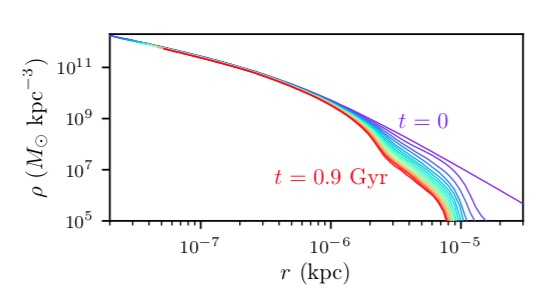
\includegraphics[width=7cm]{DensityProfileEvolutionOfHalo.jpeg}
    \caption{\cite{Delos19} Density Profile Evolution Of Halo as a function of radius at different times.}
    \label{fig:galaxy}
\end{figure}
\vspace{0.5mm}

An important question in the field is how the growth and evolution of galaxies is connected to the growth and evolution of dark matter halos. Scientists think that the Baryonic matter has a direct impact in the density profile of dark matter halo \citep{Grillo12}.
\vspace{5mm}

\section{This Project:}

In this paper we will study the change in M33’s dark matter profile owing to mass loss from MW and M31 tides and quantify the mass loss rate as a function of time.
\vspace{0.5mm}

We will be able to answer the connection of growth and evolution between the galaxy and the dark matter halo.
\vspace{0.5mm}

The galaxies are constantly changing under mass loss or gain. Analyzing how the density profile of the dark halo evolve over time owing to mass loss will describe the connection between dark matter halo and the galaxy
\vspace{5mm}

\section{Methodology:}

A plot of density profile shows how the density is distributed over some radius. Therefore, studying its evolution under some tidal forces
\vspace{0.5mm}
I will show how the density profile of M33 halo evolve over time using snapshots as MW and M31 approaches one another. 
\vspace{0.5mm}
Figure 2 below is an example of density profile using different mass ratio of dark matter halo over stellar mass. This plot comes from \cite{Conroy11} and give us more information about what the density profile of a dark matter halo look like ignoring mass loss.

\begin{figure}[h]
    \centering
    \includegraphics[width=4cm]{Densityprofilewithdifferentmassratio.jpeg}
    \caption{\cite{Conroy11} Dark Matter Halo density profile with different mass ratio.}
    \label{fig:galaxy}
\end{figure}

\vspace{0.5mm}

Using the mass enclosed over some radius (30 Kpc)  dividing by the volume we get a density. For the hernquist density, it is given From \cite{Hern90} by :

\begin{figure}[h]
    \centering
    \includegraphics[width=4cm]{HernquistDensity.jpeg}
    \caption{\cite{Hern90} Hernquist Density as a function of radius.}
    \label{fig:galaxy}
\end{figure}

We worked out plots for density profile of halo in Lab 6. Density profile will help us analyze the behavior of dark matter halo under tidal forces and mass loss. This will makes more sense as MW and M31 merge together to result in a system with a strong gravitational potential that will make M33 dark matter halo to react significantly.

\vspace{0.5mm}    

I expect the mass distribution to change fast due to mass loss and try to reach an equilibrium which will correspond to the initial trend.



\section{Result :}


The graph show the Hernquist density profile of M33 at snapshot 0, meaning our time frame. The tidal forces come mostly from M31 and is increasing as a function of time but is not enought for Halo to react significantly yet.

\begin{figure}[h]
    \centering
    \includegraphics[width=5cm]{figures/HernquistDensityProfile.png}
    \caption{(Masini, 2020) Hernquist Density Profile of M33 galaxy today.}
    \label{fig:galaxy}
\end{figure}


Figure 5 below show the density profile of the Dark Matter Halo of M33 galaxy. It is using snapshots 400 to 500 for the orbit the galaxy under the tidal influences of MW and M31, which correspond to 5.7 Gyr to 7.1 Gyr from now. Now the combined gravitational potential from the merger MW-M31 is huge and the Dark Matter Halo of M33 react immediately to the tidal forces.

\begin{figure}[h]
    \centering
    \includegraphics[width=7cm]{DensityProfileatmerge.png}
    \caption{(Masini, 2020) Density Profile Of The M33's Dark Matter Halo from 5.7 Gyr to 7.1 Gyr.}
    \label{fig:Snap400to500}
\end{figure}

Both plots have the same axis : logarithmic density in Y over a given radius in X. The density is given in Mass of the sun over spherical volume enclose using the given radius in X. The radius is given in Kilo Parsec.


\section{Discussion :}

From the graph in figure 5, we can see that M33's Dark matter halo react really fast to the MW-31 system. In fact, we calculated in the code that the merger happened to be at 6.5 Gyr which reprensent the snapshot 455. Looking at the graph we see that the trend is pretty similar from 400 to 440 and in fact, it look almost the same from snapshot 0 to 440. But at snapshot 455 the density decrease faster and faster as time goes on. Moreover, mass loss can be observed later on where the density enclosed starts at near 0.5 Kpc at snap 400 and ends up starting around 2.5 Kpc for snapshot 500.

This result confirm our expectation of the fast respond of the halo due to the tidal forces.

The figure below from \cite{Boylan2004} show the density profile of the halo core particles after a simulation of a merger at 5 Gyr. Even though the radius shown on the X axis is larger than our plot, we see the trend looks similar of our result in figure 5.

\begin{figure}[h]
    \centering
    \includegraphics[width=7cm]{DensityCoredProfile.jpeg}
    \caption{\cite{Boylan2004} Density Profile of core particles of a collision simulation at 0 and 5 Gyr, as unit of density over some radius.}
    \label{fig:galaxy}
\end{figure}

We see on figure 6 a similar trend that we got into our density profile in figure~\ref{fig:Snap400to500} from radius 2.5 Kpc to 7.5 Kpc and from 0 to about 1 h^{-1} Kpc.

In the literature, we can observe two different models of density profile. \cite{deBlok10} defined both the core and the cusp model. In the cusp model the density increase fast and is more centered at some points. The core model has a density that is approximately constant. Those models describe the way dark matter is spread inside galaxies. 

\newpage

\section{Conclusions:}

 We studied the behavior of M33's dark matter halo owing mass loss in order to have a better understanding of dark matter and galaxy evolution. 
 \vspace{0.5mm}
 
 Then we learned that tidal forces was affecting the halo and have a direct impact on his structure, the density of the halo. The density decrease like an exponential decay and look similar for about 6.5 billion years, until the MW-M31 system merge and create a strong gravitational field that perturb M33.
 \vspace{0.5mm}
 
 Exploring more about core/cusp models, we could look at the density profile of the merger (MW-M31) and see how its dark matter halo has evolved. We could also compare how the dark matter halo of M33 and the merger behave, does the mass loss from M33 halo goes into the new major halo ?

\section{Acknowledgments:}
Astropy : \cite{astropy:2018}
, matpotlib : \cite{Hunter:2007}

Numpy : \cite{Numpy}
, Python : \cite{python}

\cite{Bes}



%% For this sample we use BibTeX plus aasjournals.bst to generate the
%% the bibliography. The sample63.bib file was populated from ADS. To
%% get the citations to show in the compiled file do the following:
%%
%% pdflatex sample63.tex
%% bibtext sample63
%% pdflatex sample63.tex
%% pdflatex sample63.tex

\bibliography{citation}{}
\bibliographystyle{aasjournal}

%% This command is needed to show the entire author+affiliation list when
%% the collaboration and author truncation commands are used.  It has to
%% go at the end of the manuscript.
%\allauthors

%% Include this line if you are using the \added, \replaced, \deleted
%% commands to see a summary list of all changes at the end of the article.
%\listofchanges

\end{document}

% End of file `sample63.tex'.

To answer that question we will use the data we have on halo particles for M33 and MW-M31 and track how the density profile of M33's Dark matter halo evolve over time using a plot of density profile over time. We will need to use the center of mass class we created to keep track of the galaxies position and velocities.
\vspace{0.5mm}

I think the density of the halo should decrease until M33 collides with the new MW-M31 merger system and then the two halos will add their own Dark Matter to form a new more massive halo of Dark Matter.
\vspace{5mm}

